\documentclass[a4paper, 10pt, twoside]{article}

\usepackage[top=1in, bottom=1in, left=1in, right=1in]{geometry}
\usepackage[utf8]{inputenc}
\usepackage[spanish, es-ucroman, es-noquoting]{babel}
\usepackage{setspace}
\usepackage{fancyhdr}
\usepackage{lastpage}
\usepackage{amsmath}
\usepackage{amsfonts}
\usepackage{amsthm}
\usepackage{verbatim}
\usepackage{graphicx}
\usepackage{float}
\usepackage{enumitem} % Provee macro \setlist
\usepackage{tabularx}
\usepackage{multirow}
\usepackage{hyperref}
\usepackage{multicol}
\usepackage[toc, page]{appendix}


%%%%%%%%%% Configuración de Fancyhdr - Inicio %%%%%%%%%%
\pagestyle{fancy}
\thispagestyle{fancy}
\lhead{Trabajo Práctico 1 · Teoría de las Comunicaciones}
\rhead{Delgado · Lovisolo · Petaccio}
\renewcommand{\footrulewidth}{0.4pt}
\cfoot{\thepage /\pageref{LastPage}}

\fancypagestyle{caratula} {
   \fancyhf{}
   \cfoot{\thepage /\pageref{LastPage}}
   \renewcommand{\headrulewidth}{0pt}
   \renewcommand{\footrulewidth}{0pt}
}
%%%%%%%%%% Configuración de Fancyhdr - Fin %%%%%%%%%%


%%%%%%%%%% Miscelánea - Inicio %%%%%%%%%%
% Evita que el documento se estire verticalmente para ocupar el espacio vacío
% en cada página.
\raggedbottom

% Separación entre párrafos.
\setlength{\parskip}{0.5em}

% Separación entre elementos de listas.
\setlist{itemsep=0.5em}

% Asigna la traducción de la palabra 'Appendices'.
\renewcommand{\appendixtocname}{Apéndices}
\renewcommand{\appendixpagename}{Apéndices}
%%%%%%%%%% Miscelánea - Fin %%%%%%%%%%


%%%%%%%%%% Insertar grafo - Inicio %%%%%%%%%%
\newcommand{\grafo}[1]{
  \includegraphics[type=png,ext=.png,read=.png,width=16cm]{#1}
}
%%%%%%%%%% Insertar grafo - Fin %%%%%%%%%%


\begin{document}


%%%%%%%%%%%%%%%%%%%%%%%%%%%%%%%%%%%%%%%%%%%%%%%%%%%%%%%%%%%%%%%%%%%%%%%%%%%%%%%
%% Carátula                                                                  %%
%%%%%%%%%%%%%%%%%%%%%%%%%%%%%%%%%%%%%%%%%%%%%%%%%%%%%%%%%%%%%%%%%%%%%%%%%%%%%%%


\thispagestyle{caratula}

\begin{center}


\includegraphics[height=2cm]{DC.png} 
\hfill

\includegraphics[height=2cm]{UBA.jpg} 

\vspace{2cm}

Departamento de Computación,\\
Facultad de Ciencias Exactas y Naturales,\\
Universidad de Buenos Aires

\vspace{4cm}

\begin{Huge}
Trabajo Práctico 1
\end{Huge}

\vspace{0.5cm}

\begin{Large}
Teoría de las Comunicaciones
\end{Large}

\vspace{1cm}

Primer Cuatrimestre de 2014

\vspace{4cm}

\begin{tabular}{|c|c|c|}
\hline
Apellido y Nombre & LU & E-mail\\
\hline
Delgado, Alejandro N.  & 601/11 & nahueldelgado@gmail.com\\
Lovisolo, Leandro      & 645/11 & leandro@leandro.me\\
Petaccio, Lautaro José & 443/11 & lausuper@gmail.com\\
\hline
\end{tabular}

\end{center}

\newpage


%%%%%%%%%%%%%%%%%%%%%%%%%%%%%%%%%%%%%%%%%%%%%%%%%%%%%%%%%%%%%%%%%%%%%%%%%%%%%%%
%% Índice                                                                    %%
%%%%%%%%%%%%%%%%%%%%%%%%%%%%%%%%%%%%%%%%%%%%%%%%%%%%%%%%%%%%%%%%%%%%%%%%%%%%%%%


\tableofcontents

\newpage


%%%%%%%%%%%%%%%%%%%%%%%%%%%%%%%%%%%%%%%%%%%%%%%%%%%%%%%%%%%%%%%%%%%%%%%%%%%%%%%
%% Introducción                                                              %%
%%%%%%%%%%%%%%%%%%%%%%%%%%%%%%%%%%%%%%%%%%%%%%%%%%%%%%%%%%%%%%%%%%%%%%%%%%%%%%%


\section{Introducción téorica}
En este trabajo realizamos un análisis de redes mediante la captura de paquetes ARP.

Address Resolution Protocol (ARP) es un protocolo usado frecuentemente por las redes locales para conectar las capas 3 (capa de red) y 2 (capa de enlace) mediante la conversión o identificación de IP v4 con direcciones físicas MAC.

Existen dos tipos de paquetes posibles en el protocolo: paquetes de petición y de respuesta.
\begin{itemize}
	\item Los paquetes de petición (\textit{who-has}) son enviados mayormente en forma de broadcast con el objetivo de poder localizar la dirección MAC a la cuál le pertenece una IP conocida.
	\item Los paquetes de respuesta (\textit{is-at}) son enviados de manera uni-cast ya que se utilizan para responder a la máquina que realizó una petición con anterioridad.
\end{itemize}

La estructura de los paquetes ARP es simple, consiste principalmente de los siguientes campos:

\begin{itemize}
	\item[-] Operación - Especifica la operación que el emisor está realizando: 1 para petición, 2 para responder
	\item[-] Dirección MAC del emisor
	\item[-] Dirección IP del emisior
	\item[-] Dirección MAC del destinatario - Este campo se ignora en las peticiones
	\item[-] Dirección IP del destinatario
\end{itemize}

A continuación se describe un ejemplo de uso típico observado en la práctica.

\begin{quotation}
	Una máquina en una red quiere mandarle un paquete de datos a otra máquina en la misma red. Para esto, la máquina emisora busca en su tabla local, la dirección MAC asociada a la dirección IP a la cuál quiere mandar el paquete. Si no la encuentra, realiza el broadcasts de la petición ARP, la cual llegará eventualmente, si se encuentra conectada, a la máquina destino. La máquina destino recibirá la petición y la responderá de manera uni-cast hacia la máquina que realizó la petición, poniendo en el paquete su dirección MAC para que la máquina destino de la respuesta pueda conocer la dirección MAC que necesitaba.
\end{quotation}

El análisis de la red consiste en reconocer su topología en base al nivel de información que proveen las diferentes IP, como fuente y como destino, tomando a las IP como símbolos y estimado su probabilidad de aparición con su frecuencia muestral.


%%%%%%%%%%%%%%%%%%%%%%%%%%%%%%%%%%%%%%%%%%%%%%%%%%%%%%%%%%%%%%%%%%%%%%%%%%%%%%%
%% Desarrollo                                                                %%
%%%%%%%%%%%%%%%%%%%%%%%%%%%%%%%%%%%%%%%%%%%%%%%%%%%%%%%%%%%%%%%%%%%%%%%%%%%%%%%


\section{Desarrollo}

Implementamos, para nuestro análisis, un \textit{sniffer}\footnote{\texttt{arpsniffer.py}} o monitor de paquetes, con el objetivo de poder analizar los paquetes ARP siendo enviados vía broadcast por el medio utilizado. Esta implementación se realizó en Python y utiliza la biblioteca Scapy \footnote{\url{http://www.secdev.org/projects/scapy}} para la captura de paquetes, provista por la cátedra.

Los medios utilizados para la captura de paquetes fueron tres redes Wi-Fi, de acceso público y de frecuente utilización.

Identificamos las redes según su SSID:

\begin{itemize}
	\item Alto Palermo
	\item McDonald's
	\item Starbucks
\end{itemize}

La captura de paquetes ARP consistió en el monitoreo de los paquetes ARP durante media hora aproximadamente para cada red Wi-Fi. Se almacenaron los campos principales de cada paquete para luego realizar el análisis estadístico.

Habiendo obtenido las capturas de las redes, nos proponemos identificar el o los routers que actúan como \textit{gateway} de cada red analizada. Para esto, calculamos dos tipos de frecuencia muestral para cada IP, la primera en relación a cuántos paquetes \textit{who-has} la tienen como emisor y la segunda, cuántos paquetes \textit{who-has} la tienen como destino. De este análisis, conseguimos la frecuencia muestral de cada IP como emisor y como destino.

Para cada red consideramos las fuentes de información $S_{src}$ y $S_{dst}$ tales que sus símbolos son las direcciones IP que aparecen como origen y destino en los paquetes ARP \textit{who-has}, respectivamente. Para cada fuente, calculamos la información de cada símbolo\footnote{Es decir, cada dirección IP asociada a esa fuente de información.}.

A continuación, realizamos la identificación de el o los routers en la red utilizando la información de cada IP para ambas fuentes $S_{src}$ y $S_{dst}$. Según suponemos, las IP asociadas a los routers deberían poseer la menor cantidad de información debido a que su frecuencia de recepción e incluso emisión de paquetes ARP debería ser la más alta. Esta suposición se basa en que el router será el dispositivo a los que todos los equipos querrán comunicarse (para poder tener acceso a internet), y mantendrán su ubicación actualizada para poder realizar la comunicación.

Para obtener una visualización de la red con la que se está trabajando, graficamos las comunicaciones en la red en forma de grafos dirigidos, utilizando un script \footnote{\texttt{tgfizar.py}} en Python para representar los grafos en formato Trivial Graph Format\footnote{\url{http://en.wikipedia.org/wiki/Trivial_Graph_Format}} que luego graficamos con el software yEd\footnote{\url{http://www.yworks.com/en/products_yed_about.html}}. Tomamos como nodos los diferentes IP de ésta y como aristas dirigidas la existencia de un paquete ARP con una fuente y un destino específico.


%%%%%%%%%%%%%%%%%%%%%%%%%%%%%%%%%%%%%%%%%%%%%%%%%%%%%%%%%%%%%%%%%%%%%%%%%%%%%%%
%% Resultados                                                                %%
%%%%%%%%%%%%%%%%%%%%%%%%%%%%%%%%%%%%%%%%%%%%%%%%%%%%%%%%%%%%%%%%%%%%%%%%%%%%%%%


\section{Resultados}


%% Alto Palermo %%%%%%%%%%%%%%%%%%%%%%%%%%%%%%%%%%%%%%%%%%%%%%%%%%%%%%%%%%%%%%%


\subsection{Red \emph{Alto Palermo}}

\grafo{altopalermo}


\subsubsection{Información de los símbolos de la fuente de información $S_{src}$}

Donde $S_{src} = \{ \text{direcciones IP origen en paquetes ARP \textit{who-has}} \}$.

% GNUPLOT: LaTeX picture with Postscript
\begingroup
  \makeatletter
  \providecommand\color[2][]{%
    \GenericError{(gnuplot) \space\space\space\@spaces}{%
      Package color not loaded in conjunction with
      terminal option `colourtext'%
    }{See the gnuplot documentation for explanation.%
    }{Either use 'blacktext' in gnuplot or load the package
      color.sty in LaTeX.}%
    \renewcommand\color[2][]{}%
  }%
  \providecommand\includegraphics[2][]{%
    \GenericError{(gnuplot) \space\space\space\@spaces}{%
      Package graphicx or graphics not loaded%
    }{See the gnuplot documentation for explanation.%
    }{The gnuplot epslatex terminal needs graphicx.sty or graphics.sty.}%
    \renewcommand\includegraphics[2][]{}%
  }%
  \providecommand\rotatebox[2]{#2}%
  \@ifundefined{ifGPcolor}{%
    \newif\ifGPcolor
    \GPcolorfalse
  }{}%
  \@ifundefined{ifGPblacktext}{%
    \newif\ifGPblacktext
    \GPblacktexttrue
  }{}%
  % define a \g@addto@macro without @ in the name:
  \let\gplgaddtomacro\g@addto@macro
  % define empty templates for all commands taking text:
  \gdef\gplbacktext{}%
  \gdef\gplfronttext{}%
  \makeatother
  \ifGPblacktext
    % no textcolor at all
    \def\colorrgb#1{}%
    \def\colorgray#1{}%
  \else
    % gray or color?
    \ifGPcolor
      \def\colorrgb#1{\color[rgb]{#1}}%
      \def\colorgray#1{\color[gray]{#1}}%
      \expandafter\def\csname LTw\endcsname{\color{white}}%
      \expandafter\def\csname LTb\endcsname{\color{black}}%
      \expandafter\def\csname LTa\endcsname{\color{black}}%
      \expandafter\def\csname LT0\endcsname{\color[rgb]{1,0,0}}%
      \expandafter\def\csname LT1\endcsname{\color[rgb]{0,1,0}}%
      \expandafter\def\csname LT2\endcsname{\color[rgb]{0,0,1}}%
      \expandafter\def\csname LT3\endcsname{\color[rgb]{1,0,1}}%
      \expandafter\def\csname LT4\endcsname{\color[rgb]{0,1,1}}%
      \expandafter\def\csname LT5\endcsname{\color[rgb]{1,1,0}}%
      \expandafter\def\csname LT6\endcsname{\color[rgb]{0,0,0}}%
      \expandafter\def\csname LT7\endcsname{\color[rgb]{1,0.3,0}}%
      \expandafter\def\csname LT8\endcsname{\color[rgb]{0.5,0.5,0.5}}%
    \else
      % gray
      \def\colorrgb#1{\color{black}}%
      \def\colorgray#1{\color[gray]{#1}}%
      \expandafter\def\csname LTw\endcsname{\color{white}}%
      \expandafter\def\csname LTb\endcsname{\color{black}}%
      \expandafter\def\csname LTa\endcsname{\color{black}}%
      \expandafter\def\csname LT0\endcsname{\color{black}}%
      \expandafter\def\csname LT1\endcsname{\color{black}}%
      \expandafter\def\csname LT2\endcsname{\color{black}}%
      \expandafter\def\csname LT3\endcsname{\color{black}}%
      \expandafter\def\csname LT4\endcsname{\color{black}}%
      \expandafter\def\csname LT5\endcsname{\color{black}}%
      \expandafter\def\csname LT6\endcsname{\color{black}}%
      \expandafter\def\csname LT7\endcsname{\color{black}}%
      \expandafter\def\csname LT8\endcsname{\color{black}}%
    \fi
  \fi
  \setlength{\unitlength}{0.0500bp}%
  \begin{picture}(9000.00,4500.00)%
    \gplgaddtomacro\gplbacktext{%
      \colorrgb{0.00,0.00,0.00}%
      \put(740,240){\makebox(0,0)[r]{\strut{}0}}%
      \colorrgb{0.00,0.00,0.00}%
      \put(740,742){\makebox(0,0)[r]{\strut{}0.5}}%
      \colorrgb{0.00,0.00,0.00}%
      \put(740,1245){\makebox(0,0)[r]{\strut{}1}}%
      \colorrgb{0.00,0.00,0.00}%
      \put(740,1747){\makebox(0,0)[r]{\strut{}1.5}}%
      \colorrgb{0.00,0.00,0.00}%
      \put(740,2250){\makebox(0,0)[r]{\strut{}2}}%
      \colorrgb{0.00,0.00,0.00}%
      \put(740,2752){\makebox(0,0)[r]{\strut{}2.5}}%
      \colorrgb{0.00,0.00,0.00}%
      \put(740,3254){\makebox(0,0)[r]{\strut{}3}}%
      \colorrgb{0.00,0.00,0.00}%
      \put(740,3757){\makebox(0,0)[r]{\strut{}3.5}}%
      \colorrgb{0.00,0.00,0.00}%
      \put(740,4259){\makebox(0,0)[r]{\strut{}4}}%
      \colorrgb{0.00,0.00,0.00}%
      \put(160,2249){\rotatebox{90}{\makebox(0,0){\strut{}Entrop\'ia}}}%
    }%
    \gplgaddtomacro\gplfronttext{%
      \colorrgb{0.00,0.00,0.00}%
      \put(860,52){\rotatebox{90}{\makebox(0,0)[r]{\strut{}172.17.76.210}}}%
      \put(8639,52){\rotatebox{90}{\makebox(0,0)[r]{\strut{}172.17.0.1}}}%
    }%
    \gplbacktext
    \put(0,0){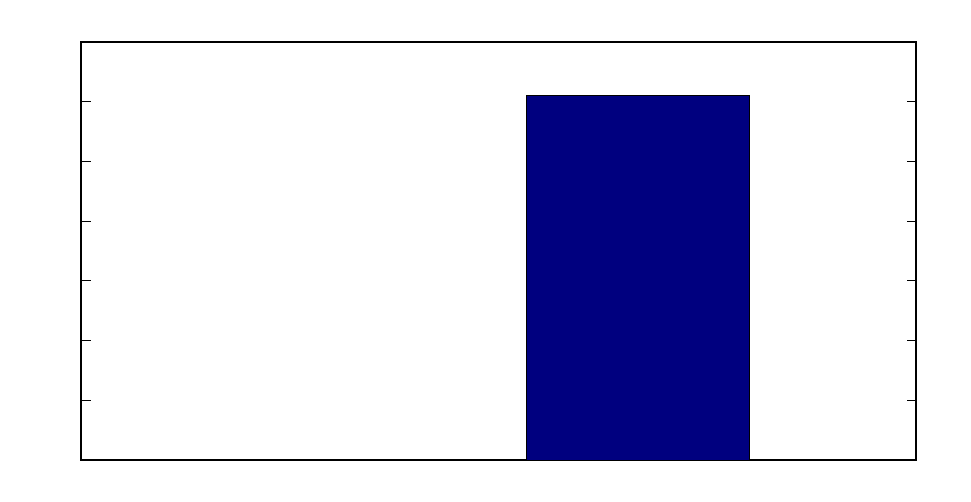
\includegraphics{altopalermo-source}}%
    \gplfronttext
  \end{picture}%
\endgroup

\vspace{2cm}


\subsubsection{Información de los símbolos de la fuente de información $S_{dst}$}

Donde $S_{dst} = \{ \text{direcciones IP destino en paquetes ARP \textit{who-has}} \}$.

% GNUPLOT: LaTeX picture with Postscript
\begingroup
  \makeatletter
  \providecommand\color[2][]{%
    \GenericError{(gnuplot) \space\space\space\@spaces}{%
      Package color not loaded in conjunction with
      terminal option `colourtext'%
    }{See the gnuplot documentation for explanation.%
    }{Either use 'blacktext' in gnuplot or load the package
      color.sty in LaTeX.}%
    \renewcommand\color[2][]{}%
  }%
  \providecommand\includegraphics[2][]{%
    \GenericError{(gnuplot) \space\space\space\@spaces}{%
      Package graphicx or graphics not loaded%
    }{See the gnuplot documentation for explanation.%
    }{The gnuplot epslatex terminal needs graphicx.sty or graphics.sty.}%
    \renewcommand\includegraphics[2][]{}%
  }%
  \providecommand\rotatebox[2]{#2}%
  \@ifundefined{ifGPcolor}{%
    \newif\ifGPcolor
    \GPcolorfalse
  }{}%
  \@ifundefined{ifGPblacktext}{%
    \newif\ifGPblacktext
    \GPblacktexttrue
  }{}%
  % define a \g@addto@macro without @ in the name:
  \let\gplgaddtomacro\g@addto@macro
  % define empty templates for all commands taking text:
  \gdef\gplbacktext{}%
  \gdef\gplfronttext{}%
  \makeatother
  \ifGPblacktext
    % no textcolor at all
    \def\colorrgb#1{}%
    \def\colorgray#1{}%
  \else
    % gray or color?
    \ifGPcolor
      \def\colorrgb#1{\color[rgb]{#1}}%
      \def\colorgray#1{\color[gray]{#1}}%
      \expandafter\def\csname LTw\endcsname{\color{white}}%
      \expandafter\def\csname LTb\endcsname{\color{black}}%
      \expandafter\def\csname LTa\endcsname{\color{black}}%
      \expandafter\def\csname LT0\endcsname{\color[rgb]{1,0,0}}%
      \expandafter\def\csname LT1\endcsname{\color[rgb]{0,1,0}}%
      \expandafter\def\csname LT2\endcsname{\color[rgb]{0,0,1}}%
      \expandafter\def\csname LT3\endcsname{\color[rgb]{1,0,1}}%
      \expandafter\def\csname LT4\endcsname{\color[rgb]{0,1,1}}%
      \expandafter\def\csname LT5\endcsname{\color[rgb]{1,1,0}}%
      \expandafter\def\csname LT6\endcsname{\color[rgb]{0,0,0}}%
      \expandafter\def\csname LT7\endcsname{\color[rgb]{1,0.3,0}}%
      \expandafter\def\csname LT8\endcsname{\color[rgb]{0.5,0.5,0.5}}%
    \else
      % gray
      \def\colorrgb#1{\color{black}}%
      \def\colorgray#1{\color[gray]{#1}}%
      \expandafter\def\csname LTw\endcsname{\color{white}}%
      \expandafter\def\csname LTb\endcsname{\color{black}}%
      \expandafter\def\csname LTa\endcsname{\color{black}}%
      \expandafter\def\csname LT0\endcsname{\color{black}}%
      \expandafter\def\csname LT1\endcsname{\color{black}}%
      \expandafter\def\csname LT2\endcsname{\color{black}}%
      \expandafter\def\csname LT3\endcsname{\color{black}}%
      \expandafter\def\csname LT4\endcsname{\color{black}}%
      \expandafter\def\csname LT5\endcsname{\color{black}}%
      \expandafter\def\csname LT6\endcsname{\color{black}}%
      \expandafter\def\csname LT7\endcsname{\color{black}}%
      \expandafter\def\csname LT8\endcsname{\color{black}}%
    \fi
  \fi
  \setlength{\unitlength}{0.0500bp}%
  \begin{picture}(9000.00,4500.00)%
    \gplgaddtomacro\gplbacktext{%
      \colorrgb{0.00,0.00,0.00}%
      \put(740,240){\makebox(0,0)[r]{\strut{}0}}%
      \colorrgb{0.00,0.00,0.00}%
      \put(740,1044){\makebox(0,0)[r]{\strut{}0.2}}%
      \colorrgb{0.00,0.00,0.00}%
      \put(740,1848){\makebox(0,0)[r]{\strut{}0.4}}%
      \colorrgb{0.00,0.00,0.00}%
      \put(740,2651){\makebox(0,0)[r]{\strut{}0.6}}%
      \colorrgb{0.00,0.00,0.00}%
      \put(740,3455){\makebox(0,0)[r]{\strut{}0.8}}%
      \colorrgb{0.00,0.00,0.00}%
      \put(740,4259){\makebox(0,0)[r]{\strut{}1}}%
      \colorrgb{0.00,0.00,0.00}%
      \put(160,2249){\rotatebox{90}{\makebox(0,0){\strut{}Entrop\'ia}}}%
    }%
    \gplgaddtomacro\gplfronttext{%
      \colorrgb{0.00,0.00,0.00}%
      \put(1148,52){\rotatebox{90}{\makebox(0,0)[r]{\strut{}172.17.88.6}}}%
      \put(1436,52){\rotatebox{90}{\makebox(0,0)[r]{\strut{}172.17.14.193}}}%
      \put(1724,52){\rotatebox{90}{\makebox(0,0)[r]{\strut{}172.17.28.173}}}%
      \put(2012,52){\rotatebox{90}{\makebox(0,0)[r]{\strut{}172.17.201.92}}}%
      \put(2301,52){\rotatebox{90}{\makebox(0,0)[r]{\strut{}172.17.8.129}}}%
      \put(2589,52){\rotatebox{90}{\makebox(0,0)[r]{\strut{}172.17.39.172}}}%
      \put(2877,52){\rotatebox{90}{\makebox(0,0)[r]{\strut{}172.17.46.252}}}%
      \put(3165,52){\rotatebox{90}{\makebox(0,0)[r]{\strut{}172.17.58.212}}}%
      \put(3453,52){\rotatebox{90}{\makebox(0,0)[r]{\strut{}172.17.0.1}}}%
      \put(3741,52){\rotatebox{90}{\makebox(0,0)[r]{\strut{}172.17.180.136}}}%
      \put(4029,52){\rotatebox{90}{\makebox(0,0)[r]{\strut{}172.17.52.76}}}%
      \put(4317,52){\rotatebox{90}{\makebox(0,0)[r]{\strut{}172.17.61.73}}}%
      \put(4605,52){\rotatebox{90}{\makebox(0,0)[r]{\strut{}172.17.41.86}}}%
      \put(4894,52){\rotatebox{90}{\makebox(0,0)[r]{\strut{}172.17.11.60}}}%
      \put(5182,52){\rotatebox{90}{\makebox(0,0)[r]{\strut{}172.17.74.1}}}%
      \put(5470,52){\rotatebox{90}{\makebox(0,0)[r]{\strut{}172.17.160.48}}}%
      \put(5758,52){\rotatebox{90}{\makebox(0,0)[r]{\strut{}172.17.9.121}}}%
      \put(6046,52){\rotatebox{90}{\makebox(0,0)[r]{\strut{}172.17.163.67}}}%
      \put(6334,52){\rotatebox{90}{\makebox(0,0)[r]{\strut{}172.17.84.225}}}%
      \put(6622,52){\rotatebox{90}{\makebox(0,0)[r]{\strut{}172.17.215.194}}}%
      \put(6910,52){\rotatebox{90}{\makebox(0,0)[r]{\strut{}172.17.167.112}}}%
      \put(7198,52){\rotatebox{90}{\makebox(0,0)[r]{\strut{}172.17.77.172}}}%
      \put(7487,52){\rotatebox{90}{\makebox(0,0)[r]{\strut{}172.17.77.135}}}%
      \put(7775,52){\rotatebox{90}{\makebox(0,0)[r]{\strut{}172.17.67.120}}}%
      \put(8063,52){\rotatebox{90}{\makebox(0,0)[r]{\strut{}172.17.60.76}}}%
      \put(8351,52){\rotatebox{90}{\makebox(0,0)[r]{\strut{}172.17.76.210}}}%
    }%
    \gplbacktext
    \put(0,0){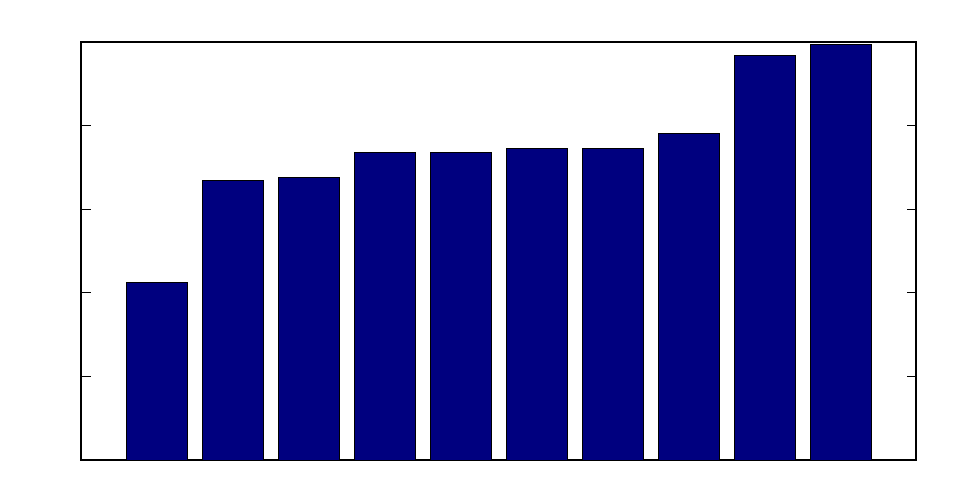
\includegraphics{altopalermo-destination}}%
    \gplfronttext
  \end{picture}%
\endgroup

\vspace{2cm}


%% McDonald's %%%%%%%%%%%%%%%%%%%%%%%%%%%%%%%%%%%%%%%%%%%%%%%%%%%%%%%%%%%%%%%%%


\subsection{Red \emph{McDonald's}}

\grafo{mcdonalds}

\grafo{mcdonalds-172.17.12.2}

\grafo{mcdonalds-172.17.12.1}

\grafo{mcdonalds-172.17.203.1}

\grafo{mcdonalds-0.0.0.0}


\subsubsection{Información de los símbolos de la fuente de información $S_{src}$}

Donde $S_{src} = \{ \text{direcciones IP origen en paquetes ARP \textit{who-has}} \}$.

% GNUPLOT: LaTeX picture with Postscript
\begingroup
  \makeatletter
  \providecommand\color[2][]{%
    \GenericError{(gnuplot) \space\space\space\@spaces}{%
      Package color not loaded in conjunction with
      terminal option `colourtext'%
    }{See the gnuplot documentation for explanation.%
    }{Either use 'blacktext' in gnuplot or load the package
      color.sty in LaTeX.}%
    \renewcommand\color[2][]{}%
  }%
  \providecommand\includegraphics[2][]{%
    \GenericError{(gnuplot) \space\space\space\@spaces}{%
      Package graphicx or graphics not loaded%
    }{See the gnuplot documentation for explanation.%
    }{The gnuplot epslatex terminal needs graphicx.sty or graphics.sty.}%
    \renewcommand\includegraphics[2][]{}%
  }%
  \providecommand\rotatebox[2]{#2}%
  \@ifundefined{ifGPcolor}{%
    \newif\ifGPcolor
    \GPcolorfalse
  }{}%
  \@ifundefined{ifGPblacktext}{%
    \newif\ifGPblacktext
    \GPblacktexttrue
  }{}%
  % define a \g@addto@macro without @ in the name:
  \let\gplgaddtomacro\g@addto@macro
  % define empty templates for all commands taking text:
  \gdef\gplbacktext{}%
  \gdef\gplfronttext{}%
  \makeatother
  \ifGPblacktext
    % no textcolor at all
    \def\colorrgb#1{}%
    \def\colorgray#1{}%
  \else
    % gray or color?
    \ifGPcolor
      \def\colorrgb#1{\color[rgb]{#1}}%
      \def\colorgray#1{\color[gray]{#1}}%
      \expandafter\def\csname LTw\endcsname{\color{white}}%
      \expandafter\def\csname LTb\endcsname{\color{black}}%
      \expandafter\def\csname LTa\endcsname{\color{black}}%
      \expandafter\def\csname LT0\endcsname{\color[rgb]{1,0,0}}%
      \expandafter\def\csname LT1\endcsname{\color[rgb]{0,1,0}}%
      \expandafter\def\csname LT2\endcsname{\color[rgb]{0,0,1}}%
      \expandafter\def\csname LT3\endcsname{\color[rgb]{1,0,1}}%
      \expandafter\def\csname LT4\endcsname{\color[rgb]{0,1,1}}%
      \expandafter\def\csname LT5\endcsname{\color[rgb]{1,1,0}}%
      \expandafter\def\csname LT6\endcsname{\color[rgb]{0,0,0}}%
      \expandafter\def\csname LT7\endcsname{\color[rgb]{1,0.3,0}}%
      \expandafter\def\csname LT8\endcsname{\color[rgb]{0.5,0.5,0.5}}%
    \else
      % gray
      \def\colorrgb#1{\color{black}}%
      \def\colorgray#1{\color[gray]{#1}}%
      \expandafter\def\csname LTw\endcsname{\color{white}}%
      \expandafter\def\csname LTb\endcsname{\color{black}}%
      \expandafter\def\csname LTa\endcsname{\color{black}}%
      \expandafter\def\csname LT0\endcsname{\color{black}}%
      \expandafter\def\csname LT1\endcsname{\color{black}}%
      \expandafter\def\csname LT2\endcsname{\color{black}}%
      \expandafter\def\csname LT3\endcsname{\color{black}}%
      \expandafter\def\csname LT4\endcsname{\color{black}}%
      \expandafter\def\csname LT5\endcsname{\color{black}}%
      \expandafter\def\csname LT6\endcsname{\color{black}}%
      \expandafter\def\csname LT7\endcsname{\color{black}}%
      \expandafter\def\csname LT8\endcsname{\color{black}}%
    \fi
  \fi
  \setlength{\unitlength}{0.0500bp}%
  \begin{picture}(9000.00,4500.00)%
    \gplgaddtomacro\gplbacktext{%
      \colorrgb{0.00,0.00,0.00}%
      \put(500,240){\makebox(0,0)[r]{\strut{}0}}%
      \colorrgb{0.00,0.00,0.00}%
      \put(500,910){\makebox(0,0)[r]{\strut{}1}}%
      \colorrgb{0.00,0.00,0.00}%
      \put(500,1580){\makebox(0,0)[r]{\strut{}2}}%
      \colorrgb{0.00,0.00,0.00}%
      \put(500,2250){\makebox(0,0)[r]{\strut{}3}}%
      \colorrgb{0.00,0.00,0.00}%
      \put(500,2919){\makebox(0,0)[r]{\strut{}4}}%
      \colorrgb{0.00,0.00,0.00}%
      \put(500,3589){\makebox(0,0)[r]{\strut{}5}}%
      \colorrgb{0.00,0.00,0.00}%
      \put(500,4259){\makebox(0,0)[r]{\strut{}6}}%
      \colorrgb{0.00,0.00,0.00}%
      \put(160,2249){\rotatebox{90}{\makebox(0,0){\strut{}Entrop\'ia}}}%
    }%
    \gplgaddtomacro\gplfronttext{%
      \colorrgb{0.00,0.00,0.00}%
      \put(728,52){\rotatebox{90}{\makebox(0,0)[r]{\strut{}172.17.12.247}}}%
      \put(837,52){\rotatebox{90}{\makebox(0,0)[r]{\strut{}172.17.12.245}}}%
      \put(945,52){\rotatebox{90}{\makebox(0,0)[r]{\strut{}172.17.203.111}}}%
      \put(1053,52){\rotatebox{90}{\makebox(0,0)[r]{\strut{}172.17.12.212}}}%
      \put(1162,52){\rotatebox{90}{\makebox(0,0)[r]{\strut{}172.17.12.38}}}%
      \put(1270,52){\rotatebox{90}{\makebox(0,0)[r]{\strut{}172.17.12.36}}}%
      \put(1379,52){\rotatebox{90}{\makebox(0,0)[r]{\strut{}10.173.104.158}}}%
      \put(1487,52){\rotatebox{90}{\makebox(0,0)[r]{\strut{}172.17.12.33}}}%
      \put(1595,52){\rotatebox{90}{\makebox(0,0)[r]{\strut{}172.17.12.31}}}%
      \put(1704,52){\rotatebox{90}{\makebox(0,0)[r]{\strut{}169.254.14.100}}}%
      \put(1812,52){\rotatebox{90}{\makebox(0,0)[r]{\strut{}172.17.12.14}}}%
      \put(1920,52){\rotatebox{90}{\makebox(0,0)[r]{\strut{}172.17.12.15}}}%
      \put(2029,52){\rotatebox{90}{\makebox(0,0)[r]{\strut{}172.17.12.73}}}%
      \put(2137,52){\rotatebox{90}{\makebox(0,0)[r]{\strut{}172.17.12.56}}}%
      \put(2245,52){\rotatebox{90}{\makebox(0,0)[r]{\strut{}172.17.12.1}}}%
      \put(2354,52){\rotatebox{90}{\makebox(0,0)[r]{\strut{}10.123.44.74}}}%
      \put(2462,52){\rotatebox{90}{\makebox(0,0)[r]{\strut{}172.17.12.4}}}%
      \put(2571,52){\rotatebox{90}{\makebox(0,0)[r]{\strut{}172.17.12.5}}}%
      \put(2679,52){\rotatebox{90}{\makebox(0,0)[r]{\strut{}169.254.159.66}}}%
      \put(2787,52){\rotatebox{90}{\makebox(0,0)[r]{\strut{}172.17.12.254}}}%
      \put(2896,52){\rotatebox{90}{\makebox(0,0)[r]{\strut{}172.17.12.253}}}%
      \put(3004,52){\rotatebox{90}{\makebox(0,0)[r]{\strut{}172.17.12.28}}}%
      \put(3112,52){\rotatebox{90}{\makebox(0,0)[r]{\strut{}172.17.12.13}}}%
      \put(3221,52){\rotatebox{90}{\makebox(0,0)[r]{\strut{}169.254.84.225}}}%
      \put(3329,52){\rotatebox{90}{\makebox(0,0)[r]{\strut{}172.17.203.107}}}%
      \put(3437,52){\rotatebox{90}{\makebox(0,0)[r]{\strut{}172.17.203.191}}}%
      \put(3546,52){\rotatebox{90}{\makebox(0,0)[r]{\strut{}172.17.12.20}}}%
      \put(3654,52){\rotatebox{90}{\makebox(0,0)[r]{\strut{}169.254.163.81}}}%
      \put(3763,52){\rotatebox{90}{\makebox(0,0)[r]{\strut{}169.254.79.68}}}%
      \put(3871,52){\rotatebox{90}{\makebox(0,0)[r]{\strut{}10.109.46.225}}}%
      \put(3979,52){\rotatebox{90}{\makebox(0,0)[r]{\strut{}100.108.113.237}}}%
      \put(4088,52){\rotatebox{90}{\makebox(0,0)[r]{\strut{}172.17.203.156}}}%
      \put(4196,52){\rotatebox{90}{\makebox(0,0)[r]{\strut{}172.17.12.40}}}%
      \put(4304,52){\rotatebox{90}{\makebox(0,0)[r]{\strut{}172.17.12.47}}}%
      \put(4413,52){\rotatebox{90}{\makebox(0,0)[r]{\strut{}172.17.12.35}}}%
      \put(4521,52){\rotatebox{90}{\makebox(0,0)[r]{\strut{}10.123.35.127}}}%
      \put(4630,52){\rotatebox{90}{\makebox(0,0)[r]{\strut{}100.75.141.85}}}%
      \put(4738,52){\rotatebox{90}{\makebox(0,0)[r]{\strut{}172.17.12.183}}}%
      \put(4846,52){\rotatebox{90}{\makebox(0,0)[r]{\strut{}172.17.12.200}}}%
      \put(4955,52){\rotatebox{90}{\makebox(0,0)[r]{\strut{}172.17.12.248}}}%
      \put(5063,52){\rotatebox{90}{\makebox(0,0)[r]{\strut{}172.17.12.239}}}%
      \put(5171,52){\rotatebox{90}{\makebox(0,0)[r]{\strut{}172.17.12.8}}}%
      \put(5280,52){\rotatebox{90}{\makebox(0,0)[r]{\strut{}172.17.12.128}}}%
      \put(5388,52){\rotatebox{90}{\makebox(0,0)[r]{\strut{}172.17.12.246}}}%
      \put(5496,52){\rotatebox{90}{\makebox(0,0)[r]{\strut{}172.17.12.240}}}%
      \put(5605,52){\rotatebox{90}{\makebox(0,0)[r]{\strut{}172.17.12.12}}}%
      \put(5713,52){\rotatebox{90}{\makebox(0,0)[r]{\strut{}172.17.12.17}}}%
      \put(5822,52){\rotatebox{90}{\makebox(0,0)[r]{\strut{}172.17.12.81}}}%
      \put(5930,52){\rotatebox{90}{\makebox(0,0)[r]{\strut{}172.17.12.189}}}%
      \put(6038,52){\rotatebox{90}{\makebox(0,0)[r]{\strut{}172.17.12.43}}}%
      \put(6147,52){\rotatebox{90}{\makebox(0,0)[r]{\strut{}172.17.12.3}}}%
      \put(6255,52){\rotatebox{90}{\makebox(0,0)[r]{\strut{}172.17.12.205}}}%
      \put(6363,52){\rotatebox{90}{\makebox(0,0)[r]{\strut{}172.17.12.11}}}%
      \put(6472,52){\rotatebox{90}{\makebox(0,0)[r]{\strut{}172.17.12.146}}}%
      \put(6580,52){\rotatebox{90}{\makebox(0,0)[r]{\strut{}172.17.12.251}}}%
      \put(6688,52){\rotatebox{90}{\makebox(0,0)[r]{\strut{}172.17.12.250}}}%
      \put(6797,52){\rotatebox{90}{\makebox(0,0)[r]{\strut{}172.17.12.19}}}%
      \put(6905,52){\rotatebox{90}{\makebox(0,0)[r]{\strut{}172.17.12.241}}}%
      \put(7014,52){\rotatebox{90}{\makebox(0,0)[r]{\strut{}172.17.12.16}}}%
      \put(7122,52){\rotatebox{90}{\makebox(0,0)[r]{\strut{}172.17.12.27}}}%
      \put(7230,52){\rotatebox{90}{\makebox(0,0)[r]{\strut{}172.17.12.203}}}%
      \put(7339,52){\rotatebox{90}{\makebox(0,0)[r]{\strut{}172.17.12.32}}}%
      \put(7447,52){\rotatebox{90}{\makebox(0,0)[r]{\strut{}172.17.12.220}}}%
      \put(7555,52){\rotatebox{90}{\makebox(0,0)[r]{\strut{}172.17.12.22}}}%
      \put(7664,52){\rotatebox{90}{\makebox(0,0)[r]{\strut{}172.17.12.237}}}%
      \put(7772,52){\rotatebox{90}{\makebox(0,0)[r]{\strut{}172.17.12.29}}}%
      \put(7880,52){\rotatebox{90}{\makebox(0,0)[r]{\strut{}172.17.12.121}}}%
      \put(7989,52){\rotatebox{90}{\makebox(0,0)[r]{\strut{}172.17.12.34}}}%
      \put(8097,52){\rotatebox{90}{\makebox(0,0)[r]{\strut{}172.17.12.219}}}%
      \put(8206,52){\rotatebox{90}{\makebox(0,0)[r]{\strut{}172.17.12.24}}}%
      \put(8314,52){\rotatebox{90}{\makebox(0,0)[r]{\strut{}172.17.12.215}}}%
      \put(8422,52){\rotatebox{90}{\makebox(0,0)[r]{\strut{}0.0.0.0}}}%
      \put(8531,52){\rotatebox{90}{\makebox(0,0)[r]{\strut{}172.17.12.2}}}%
    }%
    \gplbacktext
    \put(0,0){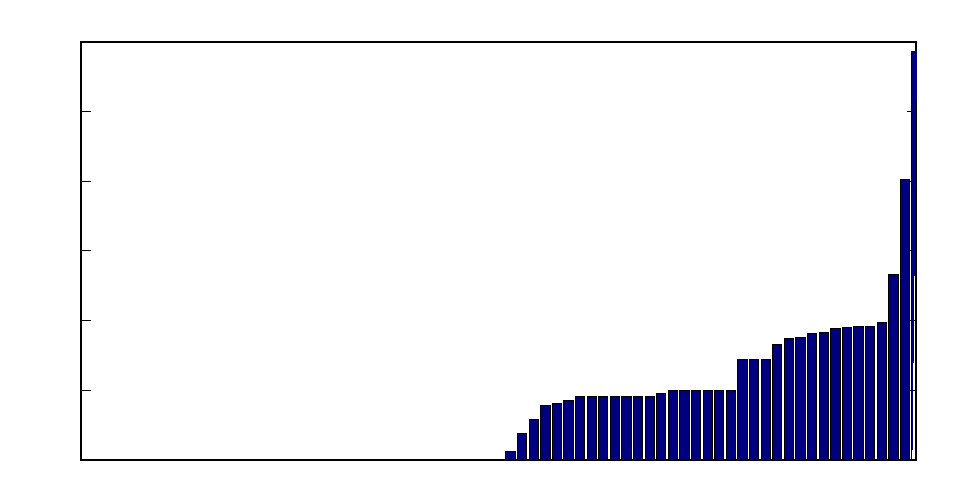
\includegraphics{mcdonalds-source}}%
    \gplfronttext
  \end{picture}%
\endgroup

\vspace{2cm}


\subsubsection{Información de los símbolos de la fuente de información $S_{dst}$}

Donde $S_{dst} = \{ \text{direcciones IP destino en paquetes ARP \textit{who-has}} \}$.

% GNUPLOT: LaTeX picture with Postscript
\begingroup
  \makeatletter
  \providecommand\color[2][]{%
    \GenericError{(gnuplot) \space\space\space\@spaces}{%
      Package color not loaded in conjunction with
      terminal option `colourtext'%
    }{See the gnuplot documentation for explanation.%
    }{Either use 'blacktext' in gnuplot or load the package
      color.sty in LaTeX.}%
    \renewcommand\color[2][]{}%
  }%
  \providecommand\includegraphics[2][]{%
    \GenericError{(gnuplot) \space\space\space\@spaces}{%
      Package graphicx or graphics not loaded%
    }{See the gnuplot documentation for explanation.%
    }{The gnuplot epslatex terminal needs graphicx.sty or graphics.sty.}%
    \renewcommand\includegraphics[2][]{}%
  }%
  \providecommand\rotatebox[2]{#2}%
  \@ifundefined{ifGPcolor}{%
    \newif\ifGPcolor
    \GPcolorfalse
  }{}%
  \@ifundefined{ifGPblacktext}{%
    \newif\ifGPblacktext
    \GPblacktexttrue
  }{}%
  % define a \g@addto@macro without @ in the name:
  \let\gplgaddtomacro\g@addto@macro
  % define empty templates for all commands taking text:
  \gdef\gplbacktext{}%
  \gdef\gplfronttext{}%
  \makeatother
  \ifGPblacktext
    % no textcolor at all
    \def\colorrgb#1{}%
    \def\colorgray#1{}%
  \else
    % gray or color?
    \ifGPcolor
      \def\colorrgb#1{\color[rgb]{#1}}%
      \def\colorgray#1{\color[gray]{#1}}%
      \expandafter\def\csname LTw\endcsname{\color{white}}%
      \expandafter\def\csname LTb\endcsname{\color{black}}%
      \expandafter\def\csname LTa\endcsname{\color{black}}%
      \expandafter\def\csname LT0\endcsname{\color[rgb]{1,0,0}}%
      \expandafter\def\csname LT1\endcsname{\color[rgb]{0,1,0}}%
      \expandafter\def\csname LT2\endcsname{\color[rgb]{0,0,1}}%
      \expandafter\def\csname LT3\endcsname{\color[rgb]{1,0,1}}%
      \expandafter\def\csname LT4\endcsname{\color[rgb]{0,1,1}}%
      \expandafter\def\csname LT5\endcsname{\color[rgb]{1,1,0}}%
      \expandafter\def\csname LT6\endcsname{\color[rgb]{0,0,0}}%
      \expandafter\def\csname LT7\endcsname{\color[rgb]{1,0.3,0}}%
      \expandafter\def\csname LT8\endcsname{\color[rgb]{0.5,0.5,0.5}}%
    \else
      % gray
      \def\colorrgb#1{\color{black}}%
      \def\colorgray#1{\color[gray]{#1}}%
      \expandafter\def\csname LTw\endcsname{\color{white}}%
      \expandafter\def\csname LTb\endcsname{\color{black}}%
      \expandafter\def\csname LTa\endcsname{\color{black}}%
      \expandafter\def\csname LT0\endcsname{\color{black}}%
      \expandafter\def\csname LT1\endcsname{\color{black}}%
      \expandafter\def\csname LT2\endcsname{\color{black}}%
      \expandafter\def\csname LT3\endcsname{\color{black}}%
      \expandafter\def\csname LT4\endcsname{\color{black}}%
      \expandafter\def\csname LT5\endcsname{\color{black}}%
      \expandafter\def\csname LT6\endcsname{\color{black}}%
      \expandafter\def\csname LT7\endcsname{\color{black}}%
      \expandafter\def\csname LT8\endcsname{\color{black}}%
    \fi
  \fi
  \setlength{\unitlength}{0.0500bp}%
  \begin{picture}(9000.00,4500.00)%
    \gplgaddtomacro\gplbacktext{%
      \colorrgb{0.00,0.00,0.00}%
      \put(500,240){\makebox(0,0)[r]{\strut{}0}}%
      \colorrgb{0.00,0.00,0.00}%
      \put(500,1044){\makebox(0,0)[r]{\strut{}1}}%
      \colorrgb{0.00,0.00,0.00}%
      \put(500,1848){\makebox(0,0)[r]{\strut{}2}}%
      \colorrgb{0.00,0.00,0.00}%
      \put(500,2651){\makebox(0,0)[r]{\strut{}3}}%
      \colorrgb{0.00,0.00,0.00}%
      \put(500,3455){\makebox(0,0)[r]{\strut{}4}}%
      \colorrgb{0.00,0.00,0.00}%
      \put(500,4259){\makebox(0,0)[r]{\strut{}5}}%
      \colorrgb{0.00,0.00,0.00}%
      \put(160,2249){\rotatebox{90}{\makebox(0,0){\strut{}Entrop\'ia}}}%
    }%
    \gplgaddtomacro\gplfronttext{%
      \colorrgb{0.00,0.00,0.00}%
      \put(708,52){\rotatebox{90}{\makebox(0,0)[r]{\strut{}172.17.12.56}}}%
      \put(796,52){\rotatebox{90}{\makebox(0,0)[r]{\strut{}172.17.12.189}}}%
      \put(884,52){\rotatebox{90}{\makebox(0,0)[r]{\strut{}172.17.12.48}}}%
      \put(972,52){\rotatebox{90}{\makebox(0,0)[r]{\strut{}172.17.12.47}}}%
      \put(1061,52){\rotatebox{90}{\makebox(0,0)[r]{\strut{}172.17.12.45}}}%
      \put(1149,52){\rotatebox{90}{\makebox(0,0)[r]{\strut{}172.17.12.44}}}%
      \put(1237,52){\rotatebox{90}{\makebox(0,0)[r]{\strut{}172.17.12.42}}}%
      \put(1325,52){\rotatebox{90}{\makebox(0,0)[r]{\strut{}172.17.12.41}}}%
      \put(1413,52){\rotatebox{90}{\makebox(0,0)[r]{\strut{}172.17.12.40}}}%
      \put(1501,52){\rotatebox{90}{\makebox(0,0)[r]{\strut{}172.17.12.203}}}%
      \put(1589,52){\rotatebox{90}{\makebox(0,0)[r]{\strut{}169.254.241.64}}}%
      \put(1677,52){\rotatebox{90}{\makebox(0,0)[r]{\strut{}50.22.225.66}}}%
      \put(1766,52){\rotatebox{90}{\makebox(0,0)[r]{\strut{}172.17.12.8}}}%
      \put(1854,52){\rotatebox{90}{\makebox(0,0)[r]{\strut{}172.17.12.9}}}%
      \put(1942,52){\rotatebox{90}{\makebox(0,0)[r]{\strut{}172.17.12.6}}}%
      \put(2030,52){\rotatebox{90}{\makebox(0,0)[r]{\strut{}172.17.12.7}}}%
      \put(2118,52){\rotatebox{90}{\makebox(0,0)[r]{\strut{}172.17.12.5}}}%
      \put(2206,52){\rotatebox{90}{\makebox(0,0)[r]{\strut{}172.17.12.3}}}%
      \put(2294,52){\rotatebox{90}{\makebox(0,0)[r]{\strut{}173.194.42.35}}}%
      \put(2382,52){\rotatebox{90}{\makebox(0,0)[r]{\strut{}172.17.203.2}}}%
      \put(2471,52){\rotatebox{90}{\makebox(0,0)[r]{\strut{}74.125.21.95}}}%
      \put(2559,52){\rotatebox{90}{\makebox(0,0)[r]{\strut{}54.207.65.66}}}%
      \put(2647,52){\rotatebox{90}{\makebox(0,0)[r]{\strut{}173.192.222.176}}}%
      \put(2735,52){\rotatebox{90}{\makebox(0,0)[r]{\strut{}169.254.144.159}}}%
      \put(2823,52){\rotatebox{90}{\makebox(0,0)[r]{\strut{}69.171.235.48}}}%
      \put(2911,52){\rotatebox{90}{\makebox(0,0)[r]{\strut{}172.17.12.10}}}%
      \put(2999,52){\rotatebox{90}{\makebox(0,0)[r]{\strut{}172.17.12.11}}}%
      \put(3087,52){\rotatebox{90}{\makebox(0,0)[r]{\strut{}172.17.12.12}}}%
      \put(3176,52){\rotatebox{90}{\makebox(0,0)[r]{\strut{}172.17.12.13}}}%
      \put(3264,52){\rotatebox{90}{\makebox(0,0)[r]{\strut{}172.17.12.14}}}%
      \put(3352,52){\rotatebox{90}{\makebox(0,0)[r]{\strut{}172.17.12.15}}}%
      \put(3440,52){\rotatebox{90}{\makebox(0,0)[r]{\strut{}172.17.12.17}}}%
      \put(3528,52){\rotatebox{90}{\makebox(0,0)[r]{\strut{}172.17.12.18}}}%
      \put(3616,52){\rotatebox{90}{\makebox(0,0)[r]{\strut{}172.17.12.19}}}%
      \put(3704,52){\rotatebox{90}{\makebox(0,0)[r]{\strut{}169.254.54.153}}}%
      \put(3792,52){\rotatebox{90}{\makebox(0,0)[r]{\strut{}172.17.12.239}}}%
      \put(3880,52){\rotatebox{90}{\makebox(0,0)[r]{\strut{}172.17.12.237}}}%
      \put(3969,52){\rotatebox{90}{\makebox(0,0)[r]{\strut{}172.17.12.128}}}%
      \put(4057,52){\rotatebox{90}{\makebox(0,0)[r]{\strut{}172.17.12.121}}}%
      \put(4145,52){\rotatebox{90}{\makebox(0,0)[r]{\strut{}172.17.12.254}}}%
      \put(4233,52){\rotatebox{90}{\makebox(0,0)[r]{\strut{}172.17.12.250}}}%
      \put(4321,52){\rotatebox{90}{\makebox(0,0)[r]{\strut{}172.17.12.253}}}%
      \put(4409,52){\rotatebox{90}{\makebox(0,0)[r]{\strut{}172.17.12.252}}}%
      \put(4497,52){\rotatebox{90}{\makebox(0,0)[r]{\strut{}172.17.12.220}}}%
      \put(4585,52){\rotatebox{90}{\makebox(0,0)[r]{\strut{}172.17.12.249}}}%
      \put(4674,52){\rotatebox{90}{\makebox(0,0)[r]{\strut{}172.17.12.247}}}%
      \put(4762,52){\rotatebox{90}{\makebox(0,0)[r]{\strut{}172.17.12.244}}}%
      \put(4850,52){\rotatebox{90}{\makebox(0,0)[r]{\strut{}172.17.12.245}}}%
      \put(4938,52){\rotatebox{90}{\makebox(0,0)[r]{\strut{}172.17.12.242}}}%
      \put(5026,52){\rotatebox{90}{\makebox(0,0)[r]{\strut{}172.17.12.243}}}%
      \put(5114,52){\rotatebox{90}{\makebox(0,0)[r]{\strut{}172.17.12.38}}}%
      \put(5202,52){\rotatebox{90}{\makebox(0,0)[r]{\strut{}172.17.12.39}}}%
      \put(5290,52){\rotatebox{90}{\makebox(0,0)[r]{\strut{}172.17.12.36}}}%
      \put(5379,52){\rotatebox{90}{\makebox(0,0)[r]{\strut{}172.17.12.35}}}%
      \put(5467,52){\rotatebox{90}{\makebox(0,0)[r]{\strut{}172.17.12.31}}}%
      \put(5555,52){\rotatebox{90}{\makebox(0,0)[r]{\strut{}172.17.12.28}}}%
      \put(5643,52){\rotatebox{90}{\makebox(0,0)[r]{\strut{}172.17.12.21}}}%
      \put(5731,52){\rotatebox{90}{\makebox(0,0)[r]{\strut{}172.17.12.20}}}%
      \put(5819,52){\rotatebox{90}{\makebox(0,0)[r]{\strut{}172.17.12.23}}}%
      \put(5907,52){\rotatebox{90}{\makebox(0,0)[r]{\strut{}172.17.12.26}}}%
      \put(5995,52){\rotatebox{90}{\makebox(0,0)[r]{\strut{}172.17.12.81}}}%
      \put(6083,52){\rotatebox{90}{\makebox(0,0)[r]{\strut{}172.17.12.46}}}%
      \put(6172,52){\rotatebox{90}{\makebox(0,0)[r]{\strut{}172.17.12.251}}}%
      \put(6260,52){\rotatebox{90}{\makebox(0,0)[r]{\strut{}169.254.79.68}}}%
      \put(6348,52){\rotatebox{90}{\makebox(0,0)[r]{\strut{}172.17.203.1}}}%
      \put(6436,52){\rotatebox{90}{\makebox(0,0)[r]{\strut{}172.17.12.219}}}%
      \put(6524,52){\rotatebox{90}{\makebox(0,0)[r]{\strut{}172.17.12.94}}}%
      \put(6612,52){\rotatebox{90}{\makebox(0,0)[r]{\strut{}172.17.12.240}}}%
      \put(6700,52){\rotatebox{90}{\makebox(0,0)[r]{\strut{}172.17.12.37}}}%
      \put(6788,52){\rotatebox{90}{\makebox(0,0)[r]{\strut{}172.17.12.248}}}%
      \put(6877,52){\rotatebox{90}{\makebox(0,0)[r]{\strut{}169.254.163.81}}}%
      \put(6965,52){\rotatebox{90}{\makebox(0,0)[r]{\strut{}172.17.12.4}}}%
      \put(7053,52){\rotatebox{90}{\makebox(0,0)[r]{\strut{}172.17.12.25}}}%
      \put(7141,52){\rotatebox{90}{\makebox(0,0)[r]{\strut{}169.254.159.66}}}%
      \put(7229,52){\rotatebox{90}{\makebox(0,0)[r]{\strut{}169.254.14.100}}}%
      \put(7317,52){\rotatebox{90}{\makebox(0,0)[r]{\strut{}169.254.84.225}}}%
      \put(7405,52){\rotatebox{90}{\makebox(0,0)[r]{\strut{}172.17.12.24}}}%
      \put(7493,52){\rotatebox{90}{\makebox(0,0)[r]{\strut{}172.17.12.241}}}%
      \put(7582,52){\rotatebox{90}{\makebox(0,0)[r]{\strut{}172.17.12.246}}}%
      \put(7670,52){\rotatebox{90}{\makebox(0,0)[r]{\strut{}172.17.12.43}}}%
      \put(7758,52){\rotatebox{90}{\makebox(0,0)[r]{\strut{}172.17.12.16}}}%
      \put(7846,52){\rotatebox{90}{\makebox(0,0)[r]{\strut{}172.17.12.32}}}%
      \put(7934,52){\rotatebox{90}{\makebox(0,0)[r]{\strut{}172.17.12.29}}}%
      \put(8022,52){\rotatebox{90}{\makebox(0,0)[r]{\strut{}172.17.12.22}}}%
      \put(8110,52){\rotatebox{90}{\makebox(0,0)[r]{\strut{}172.17.12.27}}}%
      \put(8198,52){\rotatebox{90}{\makebox(0,0)[r]{\strut{}172.17.12.34}}}%
      \put(8287,52){\rotatebox{90}{\makebox(0,0)[r]{\strut{}172.17.12.215}}}%
      \put(8375,52){\rotatebox{90}{\makebox(0,0)[r]{\strut{}169.254.255.255}}}%
      \put(8463,52){\rotatebox{90}{\makebox(0,0)[r]{\strut{}172.17.12.1}}}%
      \put(8551,52){\rotatebox{90}{\makebox(0,0)[r]{\strut{}172.17.12.2}}}%
    }%
    \gplbacktext
    \put(0,0){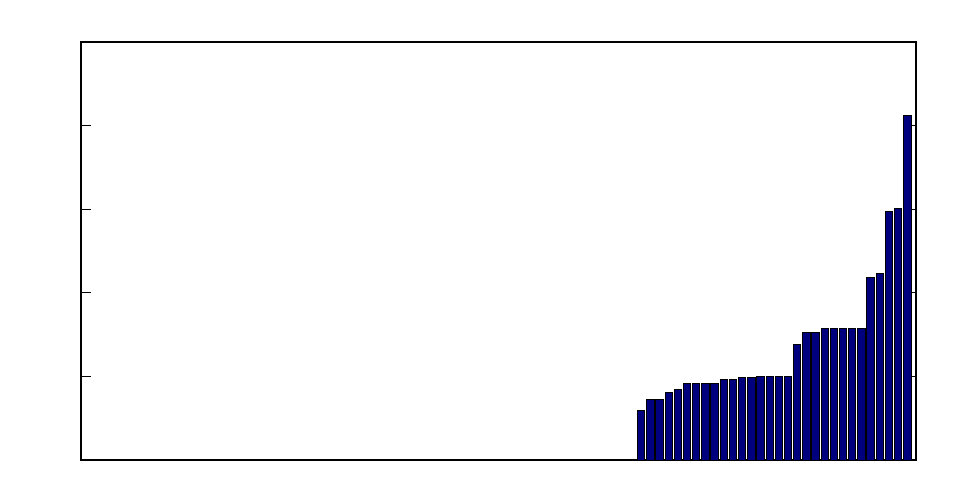
\includegraphics{mcdonalds-destination}}%
    \gplfronttext
  \end{picture}%
\endgroup

\vspace{2cm}


%% Starbucks %%%%%%%%%%%%%%%%%%%%%%%%%%%%%%%%%%%%%%%%%%%%%%%%%%%%%%%%%%%%%%%%%%


\subsection{Red \emph{Starbucks}}

\grafo{starbucks}


\subsubsection{Información de los símbolos de la fuente de información $S_{src}$}

Donde $S_{src} = \{ \text{direcciones IP origen en paquetes ARP \textit{who-has}} \}$.

% GNUPLOT: LaTeX picture with Postscript
\begingroup
  \makeatletter
  \providecommand\color[2][]{%
    \GenericError{(gnuplot) \space\space\space\@spaces}{%
      Package color not loaded in conjunction with
      terminal option `colourtext'%
    }{See the gnuplot documentation for explanation.%
    }{Either use 'blacktext' in gnuplot or load the package
      color.sty in LaTeX.}%
    \renewcommand\color[2][]{}%
  }%
  \providecommand\includegraphics[2][]{%
    \GenericError{(gnuplot) \space\space\space\@spaces}{%
      Package graphicx or graphics not loaded%
    }{See the gnuplot documentation for explanation.%
    }{The gnuplot epslatex terminal needs graphicx.sty or graphics.sty.}%
    \renewcommand\includegraphics[2][]{}%
  }%
  \providecommand\rotatebox[2]{#2}%
  \@ifundefined{ifGPcolor}{%
    \newif\ifGPcolor
    \GPcolorfalse
  }{}%
  \@ifundefined{ifGPblacktext}{%
    \newif\ifGPblacktext
    \GPblacktexttrue
  }{}%
  % define a \g@addto@macro without @ in the name:
  \let\gplgaddtomacro\g@addto@macro
  % define empty templates for all commands taking text:
  \gdef\gplbacktext{}%
  \gdef\gplfronttext{}%
  \makeatother
  \ifGPblacktext
    % no textcolor at all
    \def\colorrgb#1{}%
    \def\colorgray#1{}%
  \else
    % gray or color?
    \ifGPcolor
      \def\colorrgb#1{\color[rgb]{#1}}%
      \def\colorgray#1{\color[gray]{#1}}%
      \expandafter\def\csname LTw\endcsname{\color{white}}%
      \expandafter\def\csname LTb\endcsname{\color{black}}%
      \expandafter\def\csname LTa\endcsname{\color{black}}%
      \expandafter\def\csname LT0\endcsname{\color[rgb]{1,0,0}}%
      \expandafter\def\csname LT1\endcsname{\color[rgb]{0,1,0}}%
      \expandafter\def\csname LT2\endcsname{\color[rgb]{0,0,1}}%
      \expandafter\def\csname LT3\endcsname{\color[rgb]{1,0,1}}%
      \expandafter\def\csname LT4\endcsname{\color[rgb]{0,1,1}}%
      \expandafter\def\csname LT5\endcsname{\color[rgb]{1,1,0}}%
      \expandafter\def\csname LT6\endcsname{\color[rgb]{0,0,0}}%
      \expandafter\def\csname LT7\endcsname{\color[rgb]{1,0.3,0}}%
      \expandafter\def\csname LT8\endcsname{\color[rgb]{0.5,0.5,0.5}}%
    \else
      % gray
      \def\colorrgb#1{\color{black}}%
      \def\colorgray#1{\color[gray]{#1}}%
      \expandafter\def\csname LTw\endcsname{\color{white}}%
      \expandafter\def\csname LTb\endcsname{\color{black}}%
      \expandafter\def\csname LTa\endcsname{\color{black}}%
      \expandafter\def\csname LT0\endcsname{\color{black}}%
      \expandafter\def\csname LT1\endcsname{\color{black}}%
      \expandafter\def\csname LT2\endcsname{\color{black}}%
      \expandafter\def\csname LT3\endcsname{\color{black}}%
      \expandafter\def\csname LT4\endcsname{\color{black}}%
      \expandafter\def\csname LT5\endcsname{\color{black}}%
      \expandafter\def\csname LT6\endcsname{\color{black}}%
      \expandafter\def\csname LT7\endcsname{\color{black}}%
      \expandafter\def\csname LT8\endcsname{\color{black}}%
    \fi
  \fi
  \setlength{\unitlength}{0.0500bp}%
  \begin{picture}(9000.00,4500.00)%
    \gplgaddtomacro\gplbacktext{%
      \colorrgb{0.00,0.00,0.00}%
      \put(500,240){\makebox(0,0)[r]{\strut{}0}}%
      \colorrgb{0.00,0.00,0.00}%
      \put(500,1044){\makebox(0,0)[r]{\strut{}1}}%
      \colorrgb{0.00,0.00,0.00}%
      \put(500,1848){\makebox(0,0)[r]{\strut{}2}}%
      \colorrgb{0.00,0.00,0.00}%
      \put(500,2651){\makebox(0,0)[r]{\strut{}3}}%
      \colorrgb{0.00,0.00,0.00}%
      \put(500,3455){\makebox(0,0)[r]{\strut{}4}}%
      \colorrgb{0.00,0.00,0.00}%
      \put(500,4259){\makebox(0,0)[r]{\strut{}5}}%
      \colorrgb{0.00,0.00,0.00}%
      \put(160,2249){\rotatebox{90}{\makebox(0,0){\strut{}Informaci\'on}}}%
    }%
    \gplgaddtomacro\gplfronttext{%
      \colorrgb{0.00,0.00,0.00}%
      \put(1349,52){\rotatebox{90}{\makebox(0,0)[r]{\strut{}10.254.31.1}}}%
      \put(2078,52){\rotatebox{90}{\makebox(0,0)[r]{\strut{}0.0.0.0}}}%
      \put(2807,52){\rotatebox{90}{\makebox(0,0)[r]{\strut{}10.254.31.35}}}%
      \put(3536,52){\rotatebox{90}{\makebox(0,0)[r]{\strut{}10.254.31.42}}}%
      \put(4265,52){\rotatebox{90}{\makebox(0,0)[r]{\strut{}10.254.31.114}}}%
      \put(4994,52){\rotatebox{90}{\makebox(0,0)[r]{\strut{}10.254.31.17}}}%
      \put(5723,52){\rotatebox{90}{\makebox(0,0)[r]{\strut{}10.254.31.15}}}%
      \put(6452,52){\rotatebox{90}{\makebox(0,0)[r]{\strut{}10.254.31.68}}}%
      \put(7181,52){\rotatebox{90}{\makebox(0,0)[r]{\strut{}10.254.31.227}}}%
      \put(7910,52){\rotatebox{90}{\makebox(0,0)[r]{\strut{}10.254.31.170}}}%
    }%
    \gplbacktext
    \put(0,0){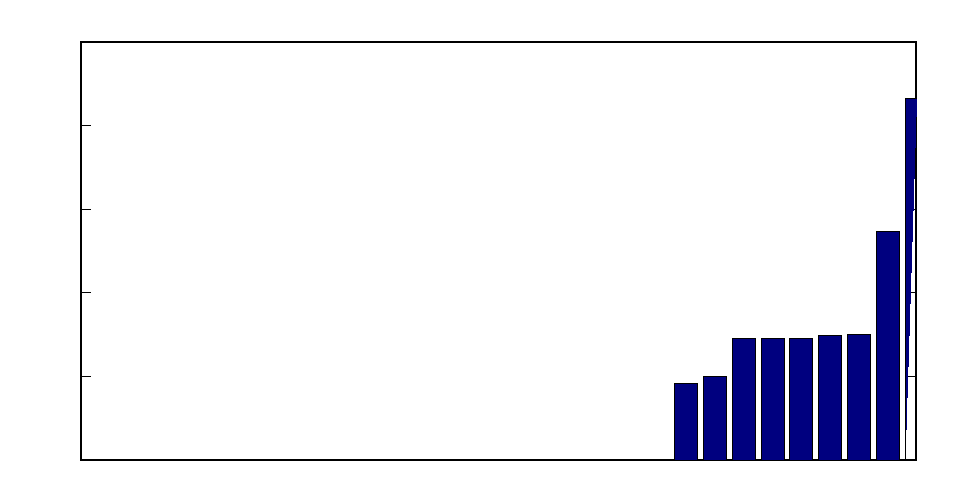
\includegraphics{starbucks-source}}%
    \gplfronttext
  \end{picture}%
\endgroup

\vspace{2cm}


\subsubsection{Información de los símbolos de la fuente de información $S_{dst}$}

Donde $S_{dst} = \{ \text{direcciones IP destino en paquetes ARP \textit{who-has}} \}$.

% GNUPLOT: LaTeX picture with Postscript
\begingroup
  \makeatletter
  \providecommand\color[2][]{%
    \GenericError{(gnuplot) \space\space\space\@spaces}{%
      Package color not loaded in conjunction with
      terminal option `colourtext'%
    }{See the gnuplot documentation for explanation.%
    }{Either use 'blacktext' in gnuplot or load the package
      color.sty in LaTeX.}%
    \renewcommand\color[2][]{}%
  }%
  \providecommand\includegraphics[2][]{%
    \GenericError{(gnuplot) \space\space\space\@spaces}{%
      Package graphicx or graphics not loaded%
    }{See the gnuplot documentation for explanation.%
    }{The gnuplot epslatex terminal needs graphicx.sty or graphics.sty.}%
    \renewcommand\includegraphics[2][]{}%
  }%
  \providecommand\rotatebox[2]{#2}%
  \@ifundefined{ifGPcolor}{%
    \newif\ifGPcolor
    \GPcolorfalse
  }{}%
  \@ifundefined{ifGPblacktext}{%
    \newif\ifGPblacktext
    \GPblacktexttrue
  }{}%
  % define a \g@addto@macro without @ in the name:
  \let\gplgaddtomacro\g@addto@macro
  % define empty templates for all commands taking text:
  \gdef\gplbacktext{}%
  \gdef\gplfronttext{}%
  \makeatother
  \ifGPblacktext
    % no textcolor at all
    \def\colorrgb#1{}%
    \def\colorgray#1{}%
  \else
    % gray or color?
    \ifGPcolor
      \def\colorrgb#1{\color[rgb]{#1}}%
      \def\colorgray#1{\color[gray]{#1}}%
      \expandafter\def\csname LTw\endcsname{\color{white}}%
      \expandafter\def\csname LTb\endcsname{\color{black}}%
      \expandafter\def\csname LTa\endcsname{\color{black}}%
      \expandafter\def\csname LT0\endcsname{\color[rgb]{1,0,0}}%
      \expandafter\def\csname LT1\endcsname{\color[rgb]{0,1,0}}%
      \expandafter\def\csname LT2\endcsname{\color[rgb]{0,0,1}}%
      \expandafter\def\csname LT3\endcsname{\color[rgb]{1,0,1}}%
      \expandafter\def\csname LT4\endcsname{\color[rgb]{0,1,1}}%
      \expandafter\def\csname LT5\endcsname{\color[rgb]{1,1,0}}%
      \expandafter\def\csname LT6\endcsname{\color[rgb]{0,0,0}}%
      \expandafter\def\csname LT7\endcsname{\color[rgb]{1,0.3,0}}%
      \expandafter\def\csname LT8\endcsname{\color[rgb]{0.5,0.5,0.5}}%
    \else
      % gray
      \def\colorrgb#1{\color{black}}%
      \def\colorgray#1{\color[gray]{#1}}%
      \expandafter\def\csname LTw\endcsname{\color{white}}%
      \expandafter\def\csname LTb\endcsname{\color{black}}%
      \expandafter\def\csname LTa\endcsname{\color{black}}%
      \expandafter\def\csname LT0\endcsname{\color{black}}%
      \expandafter\def\csname LT1\endcsname{\color{black}}%
      \expandafter\def\csname LT2\endcsname{\color{black}}%
      \expandafter\def\csname LT3\endcsname{\color{black}}%
      \expandafter\def\csname LT4\endcsname{\color{black}}%
      \expandafter\def\csname LT5\endcsname{\color{black}}%
      \expandafter\def\csname LT6\endcsname{\color{black}}%
      \expandafter\def\csname LT7\endcsname{\color{black}}%
      \expandafter\def\csname LT8\endcsname{\color{black}}%
    \fi
  \fi
  \setlength{\unitlength}{0.0500bp}%
  \begin{picture}(9000.00,4500.00)%
    \gplgaddtomacro\gplbacktext{%
      \colorrgb{0.00,0.00,0.00}%
      \put(500,240){\makebox(0,0)[r]{\strut{}0}}%
      \colorrgb{0.00,0.00,0.00}%
      \put(500,814){\makebox(0,0)[r]{\strut{}1}}%
      \colorrgb{0.00,0.00,0.00}%
      \put(500,1388){\makebox(0,0)[r]{\strut{}2}}%
      \colorrgb{0.00,0.00,0.00}%
      \put(500,1962){\makebox(0,0)[r]{\strut{}3}}%
      \colorrgb{0.00,0.00,0.00}%
      \put(500,2537){\makebox(0,0)[r]{\strut{}4}}%
      \colorrgb{0.00,0.00,0.00}%
      \put(500,3111){\makebox(0,0)[r]{\strut{}5}}%
      \colorrgb{0.00,0.00,0.00}%
      \put(500,3685){\makebox(0,0)[r]{\strut{}6}}%
      \colorrgb{0.00,0.00,0.00}%
      \put(500,4259){\makebox(0,0)[r]{\strut{}7}}%
      \colorrgb{0.00,0.00,0.00}%
      \put(160,2249){\rotatebox{90}{\makebox(0,0){\strut{}Informaci\'on}}}%
    }%
    \gplgaddtomacro\gplfronttext{%
      \colorrgb{0.00,0.00,0.00}%
      \put(1349,52){\rotatebox{90}{\makebox(0,0)[r]{\strut{}10.254.31.1}}}%
      \put(2078,52){\rotatebox{90}{\makebox(0,0)[r]{\strut{}10.254.31.42}}}%
      \put(2807,52){\rotatebox{90}{\makebox(0,0)[r]{\strut{}10.254.31.35}}}%
      \put(3536,52){\rotatebox{90}{\makebox(0,0)[r]{\strut{}169.254.255.255}}}%
      \put(4265,52){\rotatebox{90}{\makebox(0,0)[r]{\strut{}10.254.31.17}}}%
      \put(4994,52){\rotatebox{90}{\makebox(0,0)[r]{\strut{}10.254.31.15}}}%
      \put(5723,52){\rotatebox{90}{\makebox(0,0)[r]{\strut{}10.254.31.13}}}%
      \put(6452,52){\rotatebox{90}{\makebox(0,0)[r]{\strut{}169.254.151.229}}}%
      \put(7181,52){\rotatebox{90}{\makebox(0,0)[r]{\strut{}10.254.31.44}}}%
      \put(7910,52){\rotatebox{90}{\makebox(0,0)[r]{\strut{}10.254.31.41}}}%
    }%
    \gplbacktext
    \put(0,0){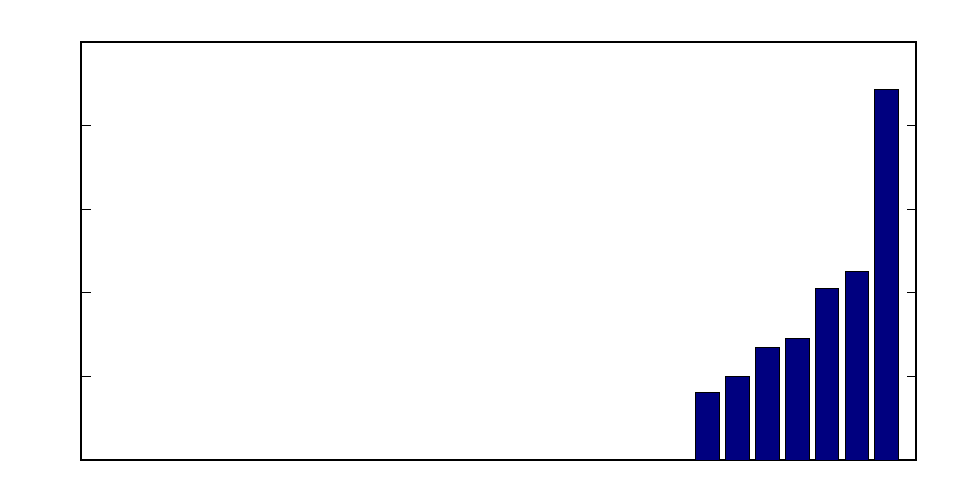
\includegraphics{starbucks-destination}}%
    \gplfronttext
  \end{picture}%
\endgroup

\vspace{2cm}


%% Entropías calculadas %%%%%%%%%%%%%%%%%%%%%%%%%%%%%%%%%%%%%%%%%%%%%%%%%%%%%%%


\subsection{Entropías calculadas}

% Constantes con la entropía calculada
\newcommand{\altopalermoSrcEntropy}{0.109542}
\newcommand{\altopalermoDstEntropy}{3.738743}
\newcommand{\mcdonaldsSrcEntropy}{3.976417}
\newcommand{\mcdonaldsDstEntropy}{3.769457}
\newcommand{\starbucksSrcEntropy}{4.142124}
\newcommand{\starbucksDstEntropy}{3.271891}


\begin{center}
\begin{tabular}{|c|c|c|}
\hline
Red & Fuente de información modelada $S$ & Entropía $H(S)$\\
\hline
Alto Palermo & $S_{src}$ & \altopalermoSrcEntropy\\
Alto Palermo & $S_{dst}$ & \altopalermoDstEntropy\\
\hline
McDonald's   & $S_{src}$ & \mcdonaldsSrcEntropy\\
McDonald's   & $S_{dst}$ & \mcdonaldsDstEntropy\\
\hline
Starbucks    & $S_{src}$ & \starbucksSrcEntropy\\
Starbucks    & $S_{dst}$ & \starbucksDstEntropy\\
\hline
\end{tabular}
\end{center}


%%%%%%%%%%%%%%%%%%%%%%%%%%%%%%%%%%%%%%%%%%%%%%%%%%%%%%%%%%%%%%%%%%%%%%%%%%%%%%%
%% Discusión                      			                                 %%
%%%%%%%%%%%%%%%%%%%%%%%%%%%%%%%%%%%%%%%%%%%%%%%%%%%%%%%%%%%%%%%%%%%%%%%%%%%%%%%


\section{Discusión}

\subsection{Fenómenos Destacables}

\subsubsection{Paquetes ARP con IP origen 0.0.0.0}

Podemos detectar en la red de McDonald's y en la de Starbucks paquetes ARP \textit{who-has} con IP origen 0.0.0.0.
El motivo de uso de esta IP es el siguiente:
Cuando un cliente se conecta a una red que posee un servidor DHCP y quiere recibir una IP de éste, manda una petición con su ID en forma de broadcast para que lo detecte el servidor. Una vez detectado por el servidor, éste manda una o varias ofertas de IP a ese ID.
El cliente eventualmente podría recibir la oferta, tomar uno de esos IP y extraer la dirección del router.
Como el servidor realiza la misma operación con todos los demás clientes que pidan una IP, el cliente debe comprobar que la IP que eligió no la tiene otro cliente. Para esto, envía un paquete \textit{who-has} con su MAC adress y la IP 0.0.0.0 como fuente para evitar confundir las ARP caches en otros hosts. Si el \textit{who-has} es respuesto, el cliente rechaza el IP elegido.

%Ver como colocar las referencias
%http://www.ietf.org/rfc/rfc2131.txt
%4.4.1


\subsubsection{Direcciones en el rango 169.254.0.0/16}

Entre los paquetes capturados detectamos varios que usaban el rango 169.254.0.0/16 como dirección IP origen o destino, el cual difiere con el rango utilizado para las IP asignadas por el servidor DHCP a los dispositivos de la red. Las direcciones en este rango se denominan \textit{direcciones de enlace local}, y son direcciones reservadas. Un host puede eventualmente asignarse una IP libre (lo corrobora con ARP) de enlace local para poder acceder de forma básica a la red cuando todavía no se le ha asignado una IP válida, ya sea de forma manual o automática (DHCP).\footnote{\url{http://tools.ietf.org/html/rfc3927}}

Esto le permite al host comunicarse con los otros dispositivos de la red, pero no con dispositivos externos a la misma.


\subsubsection{Misma IP como origen y destino}

Este escenario se presentó en muchas ocasiones, en todas las redes analizadas. Se trata de una forma de uso del protocolo llamada \textit{Gratuitous ARP}\footnote{\url{http://wiki.wireshark.org/Gratuitous_ARP}}, que existe mayormente para detectar conflictos de IP en la red, o para actualizar la información en las tablas de los vecinos.

Por ejemplo, si un host envía un Gratuitous ARP y recibe una respuesta, ya detectó un conflicto de IP, pues nadie debería responder a un request que tiene como destino el propio host.



%%%%%%%%%%%%%%%%%%%%%%%%%%%%%%%%%%%%%%%%%%%%%%%%%%%%%%%%%%%%%%%%%%%%%%%%%%%%%%%
%% Conclusión                                                                %%
%%%%%%%%%%%%%%%%%%%%%%%%%%%%%%%%%%%%%%%%%%%%%%%%%%%%%%%%%%%%%%%%%%%%%%%%%%%%%%%


\section{Conclusión}


\end{document}